\begin{frame}
    \autotitle
    \begin{itemize}
        \item
            \url{https://docs.ci.openshift.org}
            \begin{itemize}
                \item \href
                    {https://docs.ci.openshift.org/docs/architecture/ci-operator/}
                    {/docs/architecture/ci-operator}
                \item \href
                    {https://docs.ci.openshift.org/docs/internals/}
                    {/docs/internals}
                \item \href
                    {https://docs.ci.openshift.org/docs/internals/steps/}
                    {/docs/internals/steps}
            \end{itemize}
        \item
            \url{https://github.com/openshift/ci-docs/pulls}
            \begin{itemize}
                \item \href
                    {https://github.com/openshift/ci-docs/pull/233}
                    {\#233}
                \item \href
                    {https://github.com/openshift/ci-docs/pull/235}
                    {\#235}
                \item \href
                    {https://github.com/openshift/ci-docs/pull/266}
                    {\#266}
            \end{itemize}
    \end{itemize}
    \note{
        We have a few architectural descriptions of \texttt{ci-operator} and
        \texttt{ci-tools} in general.  The \texttt{architecture/ci-operator}
        page is meant for users but, since they are also developers, goes into
        fairly technical detail.  The \texttt{…-internals} page is meant for
        internal use and has abundant references to source code.

        Documenting (and understanding in the first place) is an ongoing effort,
        and there are several work-in-progress documents you can also consult.
    }
\end{frame}

\begin{frame}
    \autotitle
    \begin{center}
        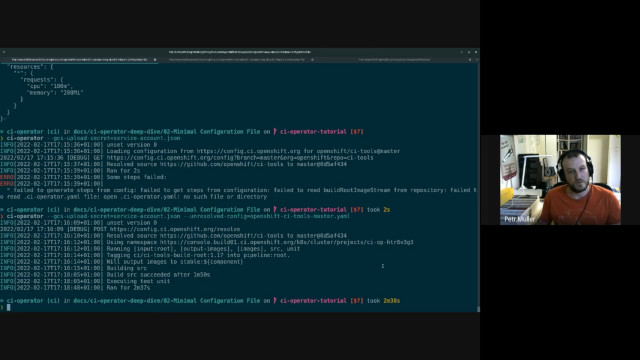
\includegraphics[scale=.4]{img/prev.jpg} \\
        \textit{Shift Week Knowledge Sharing}, Petr Muller (2022-02-17) \\
        \scriptsize
        \url{https://drive.google.com/file/d/1ye_Xim2oV4iJaQtBQrDUjre3vwDvZKDT/}
    \end{center}
    \note{
        I am going to take a different route than I normally would because we've
        already had a very good presentation by Petr in a previous knowledge
        sharing session.  It was remarkably similar to what I had in mind for a
        \texttt{ci-operator} introduction, and formed part of the basis for the
        development of \url{https://github.com/openshift/ci-docs/pull/235}.

        Instead, here we're going the opposite way, with an abstract
        architecture overview.
    }
\end{frame}

\begin{frame}
    \autotitle
    \begin{multicols}{2}
        \begin{itemize}
            \item
                Inputs
                \begin{itemize}
                    \item repository / \texttt{git} revision(s)
                    \item command-line arguments
                    \item configuration
                \end{itemize}
        \end{itemize}
        \begin{itemize}
            \item
                Outputs
                \begin{itemize}
                    \item test results
                    \item images
                \end{itemize}
        \end{itemize}
        \columnbreak
        \begin{itemize}
            \item<2>
                Implementation
                \begin{itemize}
                    \item build cluster/node
                    \item temporary namespace
                    \item image pipeline
                    \item test types
                    \item cloud providers
                    \item remote storage
                    \item image promotion
                \end{itemize}
        \end{itemize}
    \end{multicols}
    \note{
        Conceptually, the work done by \texttt{ci-operator} is relatively
        simple: it receives a list of source code references, command-line
        arguments, and a configuration file as input and produces test results
        and container images as output.  The devil is, as always, in the
        details.
    }
\end{frame}

\begin{frame}
    \autotitle
    \begin{quote}
        \texttt{ci-operator} is at its core a task scheduling program. The input
        configuration is processed and used to build a task graph, which is then
        executed until completion, failure, or interruption. Thus, the execution
        flow of \texttt{ci-operator} can be divided in these major phases:
        \begin{itemize}
            \item input processing
            \item task graph creation
            \item task graph execution
            \item cleanup
        \end{itemize}
    \end{quote}
    \note{
        This introduction from the "internals" documentation describes exactly
        what is needed to understand how \texttt{ci-operator} works.  The main
        data structure is the \textit{step graph}.
    }
\end{frame}

\begin{frame}[fragile]
    \autotitle
    \begin{verbatim}
$ ci-operator \
    --unresolved-config ci-tools-master.yaml \
    --print-graph \
    --target unit --target e2e
…
src [input:root]
test-bin src
unit src
e2e test-bin
…
    \end{verbatim} %$
    \url{https://pkg.go.dev/golang.org/x/tools/cmd/digraph}
    \note{
        There is an obscure flag which can be used to display the graph.  The
        output is meant to be used with the (equaly obscure) \texttt{digraph}
        Golang \href{https://pkg.go.dev/golang.org/x/tools/cmd/digraph}{tool}.
        Each line contains a step in the first column and its dependencies as
        subsequent columns.

        \textit{Note: some of the functionality described here (e.g. displaying
        a sub-graph with \texttt{--target}) is not yet in \texttt{master}.}
    }
\end{frame}

\begin{frame}[fragile]
    \autotitle
    \begin{verbatim}
$ ci-operator \
    --unresolved-config ci-tools-master.yaml \
    --print-graph \
    --target unit --target e2e \
    | hack/ci-operator/graphviz.pl -T png \
    > out.png
    \end{verbatim} %$
    \begin{center}
        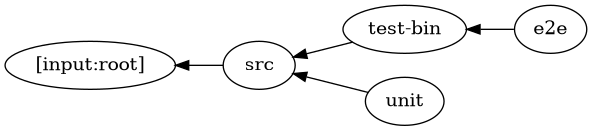
\includegraphics[scale=0.5]{img/graph.png}
        (requirement $\leftarrow$ dependent)
    \end{center}
    \note{
        With a bit of magic (a.k.a. Perl), it can be translated to the DOT
        language and visualized.
    }
\end{frame}

\begin{frame}
    \autotitle
    \begin{center}
        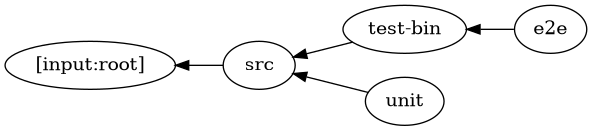
\includegraphics[scale=0.5]{img/graph.png}
    \end{center}
    \setlength\linewidth{40em}
    \setlength\columnsep{0cm}
    \begin{multicols}{2}
        \begin{itemize}
            \item import \texttt{root} image
                \begin{itemize}
                    \item \texttt{build\_root}
                    \item special name: \texttt{[input:…]}
                \end{itemize}
            \item build \texttt{src} image
                \begin{itemize}
                    \item
                        explicit requirement of \texttt{unit}, implicit
                        requirement of \texttt{test-bin}
                \end{itemize}
            \item build \texttt{test-bin} image
                \begin{itemize}
                    \item \texttt{test\_binary\_build\_commands}
                    \item
                        requested by \texttt{from:} \texttt{test-bin} in
                        \texttt{e2e}
                \end{itemize}
            \columnbreak
            \item execute \texttt{unit} test
                \begin{itemize}
                    \item \texttt{--target}
                \end{itemize}
            \item execute \texttt{e2e} test
                \begin{itemize}
                    \item \texttt{--target}
                \end{itemize}
        \end{itemize}
    \end{multicols}
\end{frame}

\begin{frame}[fragile]
    \autotitle
    \begin{verbatim}
… --target unit --target e2e --target ci-operator …
    \end{verbatim}
    \begin{center}
        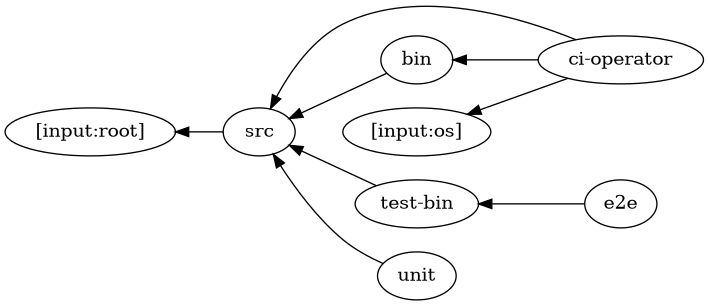
\includegraphics[scale=0.4]{img/graph_plus.png}
    \end{center}
    \note{
        If we add the \texttt{ci-operator} target to the graph (an image build),
        we can see the effect in the resulting graph:
        \begin{itemize}
            \item the previous graph is unchanged at the bottom
            \item the \texttt{ci-operator} node is added, unsurprisingly
            \item it uses an input image (\texttt{base\_images}) as a base
            \item
                it also uses the \texttt{bin} image as a base, which in turn is
                built from the \texttt{src} image
        \end{itemize}
    }
\end{frame}

\begin{frame}[fragile]
    \autotitle
    \footnotesize
    \begin{verbatim}
                                        0             0
INFO[2022-06-27T10:46:10Z] Running [input:root], [input:os], \
    src, bin, test-bin, ci-operator, unit, e2e
     1    2      2           3         2    3
    \end{verbatim}
    \begin{center}
        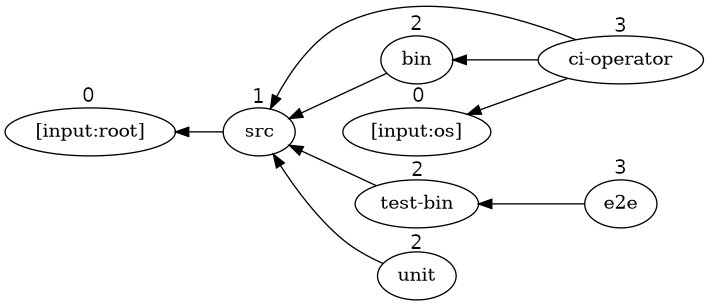
\includegraphics[scale=0.4]{img/graph_order.png}
    \end{center}
    \note{
        This graph is what the line in the \texttt{ci-operator} output which
        contains "Running" followed by a sequence of names represents: it is a
        topological order of the graph, i.e. a one-dimensional projection of the
        sequence(s) of steps to be performed.

        As described previously, these are all executed in parallel as much as
        possible, with dependent steps starting as soon as their requirements
        are satisfied.  This means this linearized version is only one of the
        possible total orders, as the dependency between steps is only a partial
        order.

        This visualization assigns a number to each node according to its
        "maximum depth" starting from the roots, giving an idea of which steps
        can be executed in parallel.
    }
\end{frame}

\begin{frame}[fragile]
    \autotitle
    \url{https://docs.ci.openshift.org/docs/internals/steps/#step-types}
    \vspace{1em}
    \begin{itemize}
        \item build steps
        \item release steps
        \item (optional) operator steps
        \item auxiliary steps
        \item test steps
        \item output steps
    \end{itemize}
    \note{
        Mastering \texttt{ci-operator} is in some sense learning the purpose and
        implementation of each type of step.  The "internals" page has sections
        for each category, with individual sub-sections for each and every step
        type.
    }
\end{frame}

\begin{frame}[fragile]
    \autotitle
    \href
        {https://github.com/openshift/ci-tools/blob/master/pkg/api/graph.go}
        {pkg/api/graph.go} (simplified)
    \begin{verbatim}
type Step interface {
    Name() string
    Description() string
    Requires() []StepLink
    Creates() []StepLink
    Inputs() (InputDefinition, error)
    Run(ctx context.Context) error
}

type StepNode struct {
    Step     Step
    Children []*StepNode
}
    \end{verbatim}
    \note{
        You can imagine what the execution code look like from that description,
        but here is a simplified version of it.  This is the step interface and
        the graph structure.
    }
\end{frame}

\begin{frame}[fragile]
    \autotitle
    \begin{verbatim}
// StepGraph is a DAG of steps referenced by
// its roots
type StepGraph []*StepNode

// OrderedStepList is a topologically-ordered
// sequence of steps.  Edges are determined
// based on the Creates/Requires methods.
type OrderedStepList []*StepNode
    \end{verbatim}
    \note{
        We have many types in \texttt{pkg/api/graph} which are all just slices
        of \texttt{StepNode} (\texttt{StepGraph}, \texttt{OrderedStepList},
        etc.).  Each is a separate type for semantic reasons.
    }
\end{frame}

\begin{frame}[fragile]
    \autotitle
    \scriptsize
    \begin{verbatim}
// TopologicalSort validates nodes form a DAG and orders them
// topologically.
func (g StepGraph) TopologicalSort() (OrderedStepList, []error) {
    …
    var waiting []*StepNode
    …
}
    \end{verbatim}
    \note{
        Here is a nice example with multiple types which are all the same
        underlying structure.
    }
\end{frame}

\begin{frame}[fragile]
    \autotitle
    \href
        {https://github.com/openshift/ci-tools/blob/master/pkg/steps/run.go}
        {pkg/steps/run.go} (simplified)
    \footnotesize
    \begin{verbatim}
func Run(graph api.StepGraph) {
    var seen []api.StepLink
    results := make(chan *api.StepNode)
    for _, root := range graph {
        go runStep(root, results)
    }
    for out := range results {
        seen = append(seen, out.Step.Creates()...)
        for _, child := range out.node.Children {
            if api.HasAllLinks(child.Step.Requires(), seen) {
                go runStep(child, results)
            }
        }
    }
}
    \end{verbatim}
    \note{
        And finally, the code which executes all steps in the graph.
    }
\end{frame}

\begin{frame}
    \autotitle
    \begin{center}
        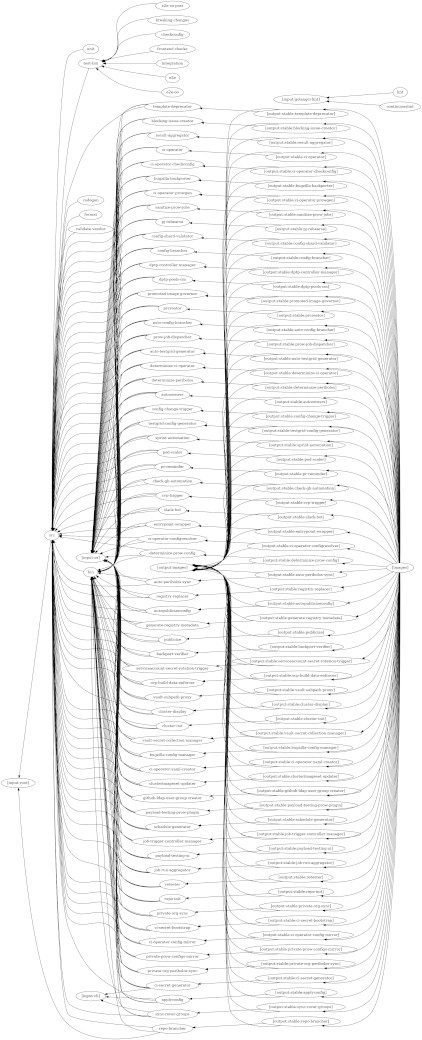
\includegraphics[height=20em]{img/ci-tools3.jpg}
    \end{center}
    \note{
        Of course, reality is \emph{much} more complicated… (this is the actual
        graph for \texttt{ci-tools}, which is still a long way from being as
        complicated as it can be)
    }
\end{frame}
